\begin{figure}[H]
\centering
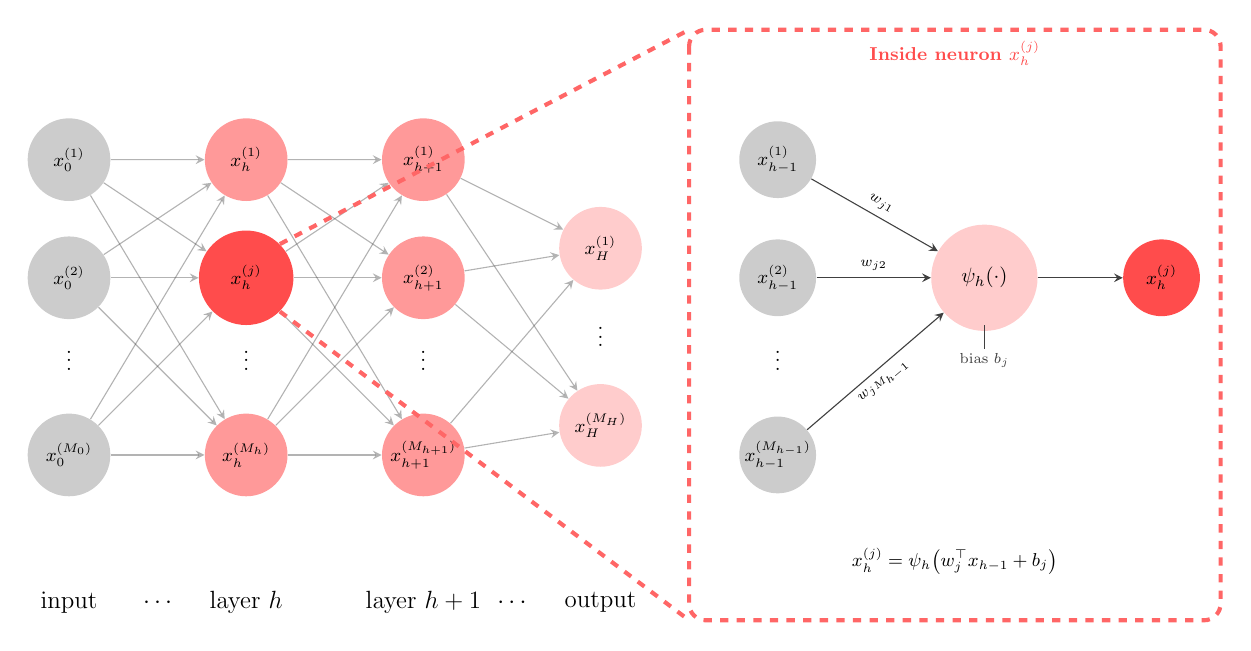
\begin{tikzpicture}[
    scale=0.75,
    transform shape,
    neuron/.style={circle, minimum size=14mm, inner sep=0pt},
    >=stealth
]
\definecolor{darkgrey}{RGB}{90,90,90}

% ======================
% Input layer (h=0)
% ======================
\node[neuron, fill=gray!40] (X01) at (0,  3.0) {\small$x_0^{(1)}$};
\node[neuron, fill=gray!40] (X02) at (0,  1.0) {\small$x_0^{(2)}$};
\node at (0, -0.3) {$\vdots$};
\node[neuron, fill=gray!40] (X0M) at (0, -2.0) {\small$x_0^{(M_0)}$};

% ======================
% Hidden layer h
% ======================
\node[neuron, fill=red!40] (Xh1) at (3,  3.0) {\small$x_h^{(1)}$};
\node[neuron, fill=red!70, minimum size=16mm] (Xhj) at (3,  1.0) {\small$x_h^{(j)}$};
\node at (3, -0.3) {$\vdots$};
\node[neuron, fill=red!40] (XhM) at (3, -2.0) {\small$x_h^{(M_h)}$};

% ======================
% Hidden layer h+1
% ======================
\node[neuron, fill=red!40] (Xh11) at (6,  3.0) {\small$x_{h+1}^{(1)}$};
\node[neuron, fill=red!40] (Xh12) at (6,  1.0) {\small$x_{h+1}^{(2)}$};
\node at (6, -0.3) {$\vdots$};
\node[neuron, fill=red!40] (Xh1M) at (6, -2.0) {\small$x_{h+1}^{(M_{h+1})}$};

% ======================
% Output layer H
% ======================
\node[neuron, fill=red!20] (XH1) at (9,  1.5) {\small$x_H^{(1)}$};
\node at (9,  0.1) {$\vdots$};
\node[neuron, fill=red!20] (XHM) at (9, -1.5) {\small$x_H^{(M_H)}$};

% ======================
% Connections
% ======================
\foreach \s in {X01,X02,X0M} {
    \foreach \t in {Xh1,Xhj,XhM} {
        \draw[->, draw=darkgray, opacity=0.4] (\s) -- (\t);
    }
}
\foreach \s in {Xh1,Xhj,XhM} {
    \foreach \t in {Xh11,Xh12,Xh1M} {
        \draw[->, draw=darkgray, opacity=0.4] (\s) -- (\t);
    }
}
\foreach \s in {Xh11,Xh12,Xh1M} {
    \foreach \t in {XH1,XHM} {
        \draw[->, draw=darkgray, opacity=0.4] (\s) -- (\t);
    }
}

% ======================
% Layer labels
% ======================
\large
\node at (0,  -4.5) {input};
\node at (1.5,-4.5) {$\cdots$};
\node at (3,  -4.5) {layer $h$};
\node at (6,  -4.5) {layer $h+1$};
\node at (7.5,-4.5) {$\cdots$};
\node at (9,  -4.5) {output};
\normalsize

% ======================
% Detail box
% ======================
\draw[dashed, red!60, rounded corners=6pt, line width=1.5pt]
    (10.5, 5.2) rectangle (19.5, -4.8);
\node[red!70, font=\small\bfseries] at (15.0, 4.8)
    {Inside neuron $x_h^{(j)}$};

% Leader lines from Xhj to detail box
\draw[dashed, red!60, line width=1.5pt] (Xhj.north east) -- (10.5,  5.2);
\draw[dashed, red!60, line width=1.5pt] (Xhj.south east) -- (10.5, -4.8);

% Mini input nodes inside detail box
\node[neuron, fill=gray!40, minimum size=13mm] (CX1) at (12.0,  3.0) {\small$x_{h-1}^{(1)}$};
\node[neuron, fill=gray!40, minimum size=13mm] (CX2) at (12.0,  1.0) {\small$x_{h-1}^{(2)}$};
\node at (12.0, -0.3) {$\vdots$};
\node[neuron, fill=gray!40, minimum size=13mm] (CXM) at (12.0, -2.0) {\small$x_{h-1}^{(M_{h-1})}$};

% Central neuron in detail box
\node[neuron, fill=red!20, minimum size=18mm] (CN) at (15.5, 1.0) {$\psi_h(\cdot)$};

% Output node in detail box
\node[neuron, fill=red!70, minimum size=13mm, font=\small, inner sep=1pt] (CO) at (18.5, 1.0) {$x_h^{(j)}$};

% Weighted arrows inside detail box
\draw[->, draw=darkgray] (CX1) -- node[above, sloped, font=\scriptsize] {$w_{j1}$} (CN);
\draw[->, draw=darkgray] (CX2) -- node[above, font=\scriptsize]         {$w_{j2}$} (CN);
\draw[->, draw=darkgray] (CXM) -- node[below, sloped, font=\scriptsize] {$w_{jM_{h-1}}$} (CN);
\draw[->, draw=darkgray] (CN)  -- (CO);

% Bias annotation
\node[font=\scriptsize, darkgray] at (15.5, -0.4) {bias $b_j$};
\draw[darkgray, thin] (15.5, -0.2) -- (15.5, 0.2);

% Equation inside detail box
\node[font=\small] at (15.0, -3.8)
    {$x_h^{(j)} = \psi_h\!\left(w_j^\top x_{h-1} + b_j\right)$};

\end{tikzpicture}
\caption{General feedforward network of depth $H$. Each node $x_h^{(j)}$
denotes the $j$-th neuron in layer $h$, for $j = 1,\ldots,M_h$.
The detail panel shows how neuron $x_h^{(j)}$ computes its output from the
previous layer $x_{h-1}$ via weights $w_j$, bias $b_j$, and
activation function $\psi_h$.}
\label{fig:nn_general}
\end{figure}